%%%%%%%%%%%%%%%%%%%%%%%%%%%%%%%%%%%%%%%%%%%%%%%%%%%%%%%%%%%%%%%%%%%%%%%%%%%%%%%%%%
\begin{frame}[fragile]\frametitle{}
\begin{center}
{\Large Naive Bayes}
\end{center}
\end{frame}

%%%%%%%%%%%%%%%%%%%%%%%%%%%%%%%%%%%%%%%%%%%%%%%%%%%%%%%%%%
\begin{frame}[fragile]\frametitle{Naive Bayes}
 What is it ?
\begin{itemize}
\item Statistical method for classification.
\item Supervised Learning Method.
\item Assumes an underlying probabilistic model, the Bayes theorem.
\item  Can solve problems involving both categorical and continuous valued attributes.
\item  Named after Thomas Bayes, who proposed the Bayes Theorem.
\end{itemize}
\end{frame}


%%%%%%%%%%%%%%%%%%%%%%%%%%%%%%%%%%%%%%%%%%%%%%%%%%%%%%%%%%%
%\begin{frame}[fragile]\frametitle{What we're trying to do}
%\begin{itemize}
%\item Model probabilistic relationships
%\item ``What is the probability that this person will get heart disease, given their diet and workout regimen?''. Output is most similar to Logistic Regression
%\end{itemize}
%\end{frame}
%
%
%%%%%%%%%%%%%%%%%%%%%%%%%%%%%%%%%%%%%%%%%%%%%%%%%%%%%%%%%%%
%\begin{frame}[fragile]\frametitle{What we're trying to do}
%Will introduce Naive Bayes model
%	\begin{itemize}
%	\item A type of Bayesian classifier
%	\item More advanced: Bayesian network
%	\end{itemize}
%\end{frame}

%%%%%%%%%%%%%%%%%%%%%%%%%%%%%%%%%%%%%%%%%%%%%%%%%%%%%%%%%%%
%\begin{frame}[fragile]\frametitle{What we're trying to do}
% Bayes Classifier
%	\begin{itemize}
%	\item A probabilistic framework for solving classification problems
%	\item Used in both naive Bayes and Bayesian networks
%	\item Based on Bayes' Theorem
%	\end{itemize}
%
%\end{frame}

%%%%%%%%%%%%%%%%%%%%%%%%%%%%%%%%%%%%%%%%%%%%%%%%%%%%%%%%%%%%%%%%%%%%%%%%%%%%%%%%%%
\begin{frame}[fragile]\frametitle{}
\begin{center}
{\Large Bayes Theorem}
\end{center}
\end{frame}


%%%%%%%%%%%%%%%%%%%%%%%%%%%%%%%%%%%%%%%%%%%%%%%%%%%%%%%%%%
\begin{frame}[fragile]\frametitle{Probability (recap)}

\begin{itemize}
\item Single Probability: ``X has the value x'' $P(X=x)$
\item Joint probability: ``X and Y'': $P(X=x, Y=y)$
\item The probability that variable X takes on the value x and variable Y has the value y: $P(X , Y)$
\item Conditional probability: ``Y'' given observation of ``X'': $P( Y=y | X=x )$
\item If ``X'' and ``Y'' are independent then $P(X , Y) = P(X) \times P(Y)$
\item For dependent ``X'' and ``Y'' : $P(X , Y) = P(Y|X) \times P(X)$
\end{itemize}

\end{frame}


%%%%%%%%%%%%%%%%%%%%%%%%%%%%%%%%%%%%%%%%%%%%%%%%%%%%%%%%%%
\begin{frame}[fragile]\frametitle{Probability (recap)}
Derivation
\begin{center}
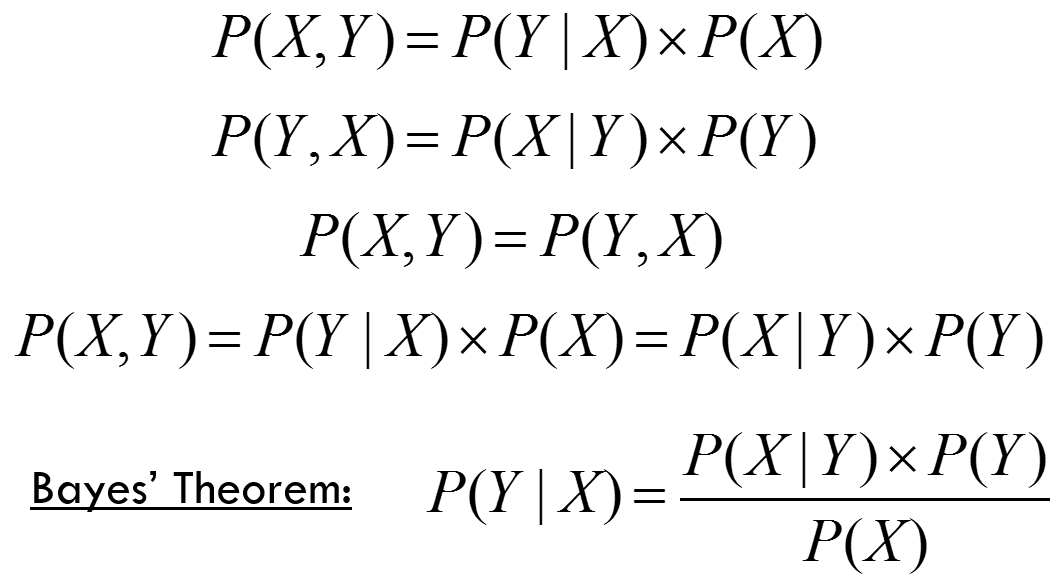
\includegraphics[width=0.8\linewidth,keepaspectratio]{nbeqs}
\end{center}
%\begin{itemize}
%\item What's the probability that it rains today and that I'm carrying an umbrella?
%\item Given that I'm observed with an umbrella, what's the probability that it will rain today?
%\end{itemize}
\end{frame}

%%%%%%%%%%%%%%%%%%%%%%%%%%%%%%%%%%%%%%%%%%%%%%%%%%%%%%%%%%
\begin{frame}[fragile]\frametitle{Example}

\begin{itemize}
\item On a college campus, you meet a guy, say ``Tom''. He appears Shy. 
\item You are asked to guess, whether Tom is a Math PhD student or a Business MBA student. Assume that these are the only two types in that campus.
\item Your guess is probably: Math PhD student, assuming that we have seen many Math PhD students, Shy.
\item Let us check if this is true, using Bayes theorem.
\end{itemize}

{\tiny (Ref: A visual guide to Bayesian thinking )}
\end{frame}

%%%%%%%%%%%%%%%%%%%%%%%%%%%%%%%%%%%%%%%%%%%%%%%%%%%%%%%%%%
\begin{frame}[fragile]\frametitle{Example}

\begin{itemize}
\item We need to see, how many Math PhD students are there? Compared to Business MBA students. Say 1: 10. This is called Prior ratio. It is the ratio if the domain or base itself in the population.
\item Within Math PhD students, you find as many as 75\% shy folks.
\item Within Business MBA students, you find just about 15\% shy folks.
\item These above to form a likelihood ratio.

\end{itemize}

{\tiny (Ref: A visual guide to Bayesian thinking )}
\end{frame}

%%%%%%%%%%%%%%%%%%%%%%%%%%%%%%%%%%%%%%%%%%%%%%%%%%%%%%%%%%
\begin{frame}[fragile]\frametitle{Example}

We need to find where Tom belongs. One thing for sure, being Shy, he must be in one of those shaded patches (shown below)


\begin{center}
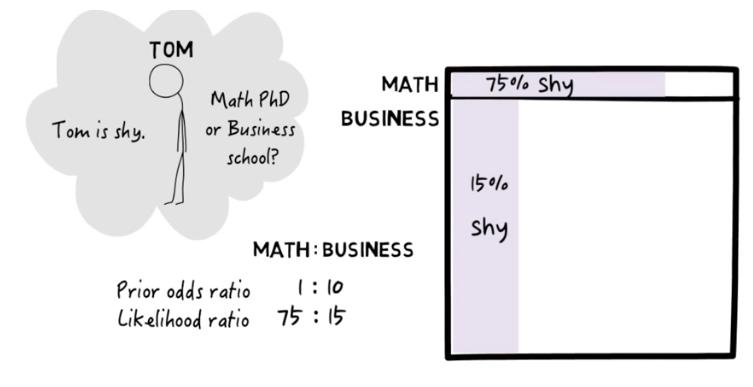
\includegraphics[width=0.8\linewidth,keepaspectratio]{nb_maths_mba}
\end{center}

Just by looking at it the Business, shaded portion looks twice the Math shaded portion. Even though individual percentages show that Math are higher. But there are higher within smaller base!!

{\tiny (Ref: A visual guide to Bayesian thinking )}
\end{frame}

%%%%%%%%%%%%%%%%%%%%%%%%%%%%%%%%%%%%%%%%%%%%%%%%%%%%%%%%%%
\begin{frame}[fragile]\frametitle{Example}

\begin{itemize}
\item If you multiply corresponding values, $1x 75 : 10 x 15$, it is $75: 150$, ie $1:2$
\item So that’s the shaded area ratio. Note that Math is in column 1, Business column 2, is 2. 
\item That’s called Posterior Probability.
\item So, Tom is more likely to be a Business MBA guy than Math PhD!!
\end{itemize}

{\tiny (Ref: A visual guide to Bayesian thinking )}
\end{frame}

%%%%%%%%%%%%%%%%%%%%%%%%%%%%%%%%%%%%%%%%%%%%%%%%%%%%%%%%%%%%%%%%%%%%%%%%%%%%%%%%%%
\begin{frame}[fragile]\frametitle{}
\begin{center}
{\Large Bayes Learning}

{\tiny (Ref: Georgia tech, Udacity, Machine Learning)}

\end{center}


\end{frame}

%%%%%%%%%%%%%%%%%%%%%%%%%%%%%%%%%%%%%%%%%%%%%%%%%%%%%%%%%%
\begin{frame}[fragile]\frametitle{Bayesian Learning}

\begin{itemize}
\item Goal of machine learning is: We want best model/function for the given data. 
\item Can we say? Its equivalent to: We want most ``probable'' model, for the given data.
\item That's represented by: $P(h|D)$ where h is hypothesis (think of it as a function) and D is data.
\item We can try many hypotheses, and find max of them.

\end{itemize}

\end{frame}

%%%%%%%%%%%%%%%%%%%%%%%%%%%%%%%%%%%%%%%%%%%%%%%%%%%%%%%%%%
\begin{frame}[fragile]\frametitle{Bayes Rule (recall)}

\begin{itemize}
\item $P(h|D) = \frac{P(D|h)P(h)}{P(D)}$
\item Chain Rule: $P(a \cap b) = P(a|b)P(b) = P(b|a)(a)$ as its symmetric
\item Better way to understand is $P(a|b)$ is probability of a given b, meaning within b, how much is a, ie the intersection of a and b. 
\item So $P(a|b)$ is $\frac{a \cap b}{b}$, right?
\end{itemize}

\end{frame}

%%%%%%%%%%%%%%%%%%%%%%%%%%%%%%%%%%%%%%%%%%%%%%%%%%%%%%%%%%
\begin{frame}[fragile]\frametitle{De-constructing the formula}

\begin{itemize}
\item The bottom term, $P(D)$ is called as Prior on the Data, ie belief of seeing the data. 
\item As we are comparing many hypotheses, and this bottom term being there in all such calculations, one can ignore it. It’s a normalization term.
\item $P(D|h)$ is like learning backwards. Its easy to see it in the machine learning dataset. Its basically the LIKELIHOOD of seeing Data given the hypothesis.
\item Note : $D = {(x_i, y_i)}$
\item So it means, given $x_i$, and the hypothesis that we are testing, meaning the function, whats the likelihood of seeing $y_i$?

\end{itemize}

\end{frame}

%%%%%%%%%%%%%%%%%%%%%%%%%%%%%%%%%%%%%%%%%%%%%%%%%%%%%%%%%%
\begin{frame}[fragile]\frametitle{Example}

\begin{itemize}
\item Hypothesis h = return true if $x > 10$
\item Data $x = 7$
\item Now the question is what is the probability of $y == True$. 
\item Its 0. 
\item What for False? 
\item Its 1.


\end{itemize}

\end{frame}

%%%%%%%%%%%%%%%%%%%%%%%%%%%%%%%%%%%%%%%%%%%%%%%%%%%%%%%%%%
\begin{frame}[fragile]\frametitle{Back to formula}

\begin{itemize}
\item As we have labeled data, its easier to compute/adjust $P(D|h)$ (as h and D are known) than $P(h|D)$
\item $P(h)$ is prior on $h$. 
\item Probability of this hypothesis $h$ occurring amongst all hypotheses. 
\item Its actually domain knowledge, the features, the type of model we are trying. 
\item It’s the probability of selected features or model.
\end{itemize}

\end{frame}



%%%%%%%%%%%%%%%%%%%%%%%%%%%%%%%%%%%%%%%%%%%%%%%%%%%%%%%%%%
\begin{frame}[fragile]\frametitle{Properties}

\begin{itemize}
\item If we have left hand side, ie ,$P(h|D)$ to go up, what should be changed on the right hand side?
\item $P(h)$ can go up. Probability of getting good hypothesis, ie better features or model, without seeing data, can go up
\item $P(D|h)$: Once you see data, for that data,  if you get that nicely predicting with $h$, then we are good. Good accuracy giving $h$.
\item $P(D)$ cannot change, (ie cannot go down)

\end{itemize}

\end{frame}

%%%%%%%%%%%%%%%%%%%%%%%%%%%%%%%%%%%%%%%%%%%%%%%%%%%%%%%%%%
\begin{frame}[fragile]\frametitle{Example}

\begin{itemize}
\item A man goes to a doctor. He gives him a test for a rare disease. The test generally returns correct positive results 98% of times and correct negative results 97\% of times.
\item $TP=0.98, TN=0.97, FP=0.02, FN=0.03$
\item The disease in general, in the population is to only .8\% people.
\item The result: the test comes positive.
\item Question: Does he really have the disease?


\end{itemize}

\end{frame}

%%%%%%%%%%%%%%%%%%%%%%%%%%%%%%%%%%%%%%%%%%%%%%%%%%%%%%%%%%
\begin{frame}[fragile]\frametitle{Example}

\begin{itemize}
\item We are looking for intersection set of $test=positive$ and $disease = true$
\item Let’s apply Bayes rule to see probability of disease being there given the test has come out positive.
\item $P(disease=true|test=positive) = \frac{P(test=positive | disease=True)P(disease=True)}{P(test=Positive)}$
\item Let’s see the probability of not having the disease even of the test said true
\item $P(disease=false|test=positive) = \frac{P(test=positive | disease=false)P(disease=False)}{P(test=Positive)}$
\item Which is bigger?
\item As you can see, for comparison, the denominators are same, so we need not calculate it.

\end{itemize}

\end{frame}


%%%%%%%%%%%%%%%%%%%%%%%%%%%%%%%%%%%%%%%%%%%%%%%%%%%%%%%%%%
\begin{frame}[fragile]\frametitle{Solution}

\begin{itemize}
\item $P(disease=true|test==positive)= 0.98 x 0.008 = 0.00784$ (ignored denominator term)
\item $P(disease=false|test==positive)= 0.03x 0.992 = 0.02976$. This is bigger. 
\item SO, don’t Panic!!
\item Just within results ie 0.00784 and 0.02976, Probability of disease not being there, is $0.02976/(0.02976+0.00784) = 0.79$, ie about 79\% probability that you won’t have disease even if the test was Positive. Only remaining 21\% chance that you may have the disease.
\end{itemize}

\end{frame}

%%%%%%%%%%%%%%%%%%%%%%%%%%%%%%%%%%%%%%%%%%%%%%%%%%%%%%%%%%
\begin{frame}[fragile]\frametitle{Algorithm}

\begin{lstlisting}
For each h in H
    Calculate p(h|D) = P(D|h)P(h)/P(D)
Output:
    H = argmax_h P(h|D)

\end{lstlisting}

\begin{itemize}
\item Good part is, as we want argmax only, we don’t need denominator P(D) , which is hard to calculate anyway.
\item $P(h)$ is also hard to compute. So if we further drop that and find $argmax P(D|h)$ than its called Maximum Likelihood Hypothesis. 
\item That just makes an assumption, that all $P(h)$ are same. 
\item All model or feature scheme are equally likely
\end{itemize}

\end{frame}

%%%%%%%%%%%%%%%%%%%%%%%%%%%%%%%%%%%%%%%%%%%%%%%%%%%%%%%%%%%%%%%%%%%%%%%%%%%%%%%%%%
\begin{frame}[fragile]\frametitle{}
\begin{center}
{\Large Bayesian Classifier}
\end{center}

\end{frame}


%%%%%%%%%%%%%%%%%%%%%%%%%%%%%%%%%%%%%%%%%%%%%%%%%%%%%%%%%%
\begin{frame}[fragile]\frametitle{Bayes Classifier}
%\begin{center}
%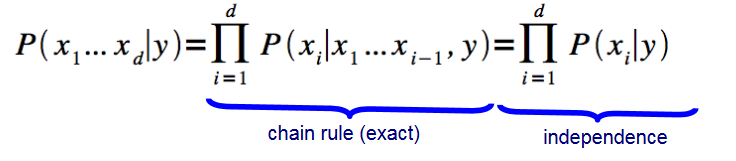
\includegraphics[width=0.6\linewidth,keepaspectratio]{nb1}
%\end{center}
	\begin{itemize}
	\item A classifier is a function
	\item It takes features as inputs, so $x_1,x_2 \ldots$
	\item Gives y as output, which could be $y=1,y=2,\ldots$. These are the classes. For binary classifier y can take only $0,1$.
	\item x can be real or numeric and it could also be categorical.
	\item With training data, the function is learnt. That's the classifier model.
	\end{itemize}

\end{frame}

%%%%%%%%%%%%%%%%%%%%%%%%%%%%%%%%%%%%%%%%%%%%%%%%%%%%%%%%%%
\begin{frame}[fragile]\frametitle{Bayes Classifier}
%\begin{center}
%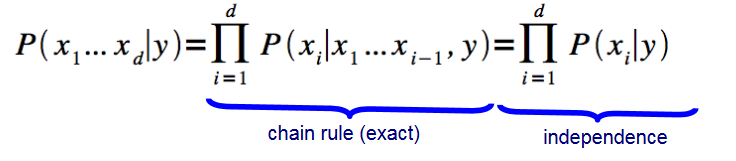
\includegraphics[width=0.6\linewidth,keepaspectratio]{nb1}
%\end{center}
	\begin{itemize}
	\item Bayesian Classifier is probabilistic.
	\item Meaning, it does not produce y class values directly,  but it gives probabilities of $y=0$ and $y=1$
	\item We pick max and say that, that's the output class
	\item $\hat{y} = arg max P (y|x)$
	\end{itemize}

\end{frame}


%%%%%%%%%%%%%%%%%%%%%%%%%%%%%%%%%%%%%%%%%%%%%%%%%%%%%%%%%%%
%\begin{frame}[fragile]\frametitle{Bayesian classification }
%Bayes Theorem: $P(Y|X) = \frac{P(X|Y)(P(Y)}{P(X)}$
%\begin{itemize}
%\item P(Y|X) : Probability that the customer will buy a computer given that 
%we know his age, credit rating and income. (Posterior Probability of Y)
%\item P(Y) : Probability that the customer will buy a computer regardless 
%of age, credit rating, income (Prior Probability of Y)
%\item P(X|Y) : Probability that the customer is 35 yrs old, have fair credit 
%rating and earns \$40,000, given that he has bought our computer 
%(Posterior Probability of X)
%\item P(X) : Probability that a person from our set of customers is 35 yrs 
%old, have fair credit rating and earns \$40,000. (Prior Probability of X). 
%\end{itemize}
%\end{frame}


%%%%%%%%%%%%%%%%%%%%%%%%%%%%%%%%%%%%%%%%%%%%%%%%%%%%%%%%%%
\begin{frame}[fragile]\frametitle{Bayesian classification }
Example
\begin{center}
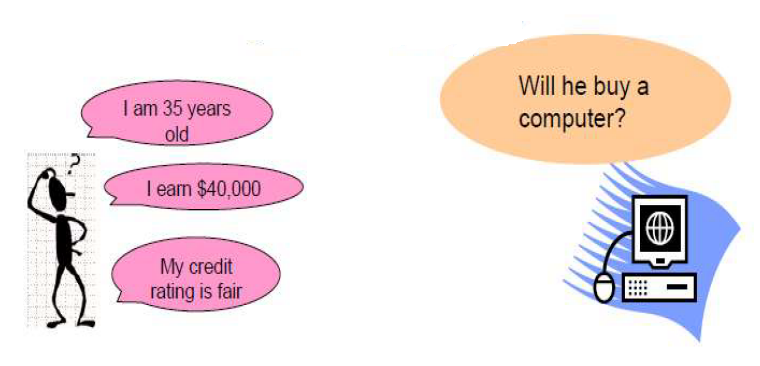
\includegraphics[width=0.6\linewidth,keepaspectratio]{nb4}
\end{center}
\begin{itemize}
\item X: Independent Variables: Age, Income, Credit Rating
\item Y: Dependent Variable: Will buy computer or not? Binary.
\end{itemize}
\end{frame}



%%%%%%%%%%%%%%%%%%%%%%%%%%%%%%%%%%%%%%%%%%%%%%%%%%%%%%%%%%
\begin{frame}[fragile]\frametitle{Bayesian classification }
%\begin{itemize}
%\item Goal: learning function: $f(x) \rightarrow y$ 
%	\begin{itemize}
%	\item $y$: one of $k$ classes (e.g. spam/ham, digit 0-9) 
%	\item $x = x_1 \ldots x_n$: values of attributes (numeric or categorical) 
%	\end{itemize}
%\item Probabilistic classification: most probable class given observation: $\hat{y} = arg~max_y P(y|x)$
%\end{itemize}
Bayesian probability of a class:
\begin{center}
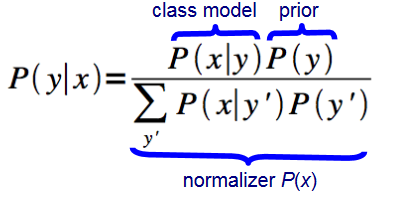
\includegraphics[width=0.6\linewidth,keepaspectratio]{nb3}
\end{center}
\begin{itemize}
\item Where denominator term of Bayes Theorem: $P(Y|X) = \frac{P(X|Y)(P(Y)}{P(X)}$ is expanded
\item Its summation of Probabilities that customer is 35 given that he buys computer, customer has fair credit rating given that he buys computer, and so on. And, also similarly for when he does not buy computer.
\end{itemize}
\end{frame}

%%%%%%%%%%%%%%%%%%%%%%%%%%%%%%%%%%%%%%%%%%%%%%%%%%%%%%%%%%
\begin{frame}[fragile]\frametitle{Bayesian classification Example}
\begin{center}
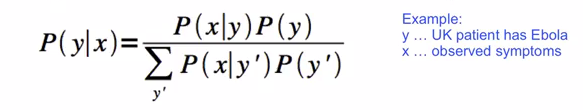
\includegraphics[width=\linewidth,keepaspectratio]{nb5}
\end{center}
\begin{itemize}
\item y is binary, whether Ebola is present or not.
\item x are many, whether s/he has temperature, looks pale, and similar symptoms.
\end{itemize}
\end{frame}

%%%%%%%%%%%%%%%%%%%%%%%%%%%%%%%%%%%%%%%%%%%%%%%%%%%%%%%%%%
\begin{frame}[fragile]\frametitle{Bayesian classification Example}
\begin{center}
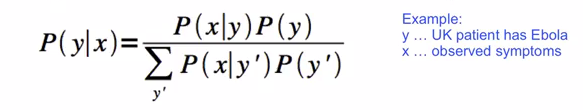
\includegraphics[width=\linewidth,keepaspectratio]{nb5}
\end{center}
\begin{itemize}
\item P(y): In general, without considering any features or symptoms, whats the probability of having Ebola.
\item Say, in general, probability of having Ebola is very less. Its rare disease in the developed world.
\item So, even if there are some symptoms, likelihood of they being for Ebola, is less. That's the role ``prior'' plays.
\end{itemize}
\end{frame}

%%%%%%%%%%%%%%%%%%%%%%%%%%%%%%%%%%%%%%%%%%%%%%%%%%%%%%%%%%
\begin{frame}[fragile]\frametitle{Bayesian classification Example}
\begin{center}
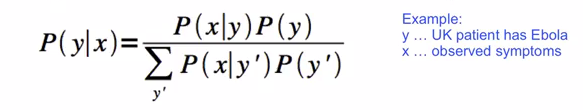
\includegraphics[width=\linewidth,keepaspectratio]{nb5}
\end{center}
\begin{itemize}
\item $P(x|y)$: Given that he has Ebola, within this sub population, what are the chances of he having x symptom.
\item Gen that he has Ebola how probable is he having (high) temperature. 
\item Similarly for other symptoms, or Xs
\end{itemize}
\end{frame}

%%%%%%%%%%%%%%%%%%%%%%%%%%%%%%%%%%%%%%%%%%%%%%%%%%%%%%%%%%
\begin{frame}[fragile]\frametitle{Bayesian classification Example}
\begin{center}
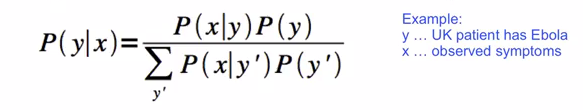
\includegraphics[width=\linewidth,keepaspectratio]{nb5}
\end{center}
\begin{itemize}
\item P(x): It is summation of having certain symptom.
\item Its sum of having this symptom with Ebola and not having Eblola
\item $P(X) = P(X|y=Ebola)P(y=Ebola) + P(X|y=NoEbola)P(y=NoEbola)$ 
\item Many a times, this term is left out from the formula, as it does not take part in the classification.
\item Because, regardless of whether the guy has Ebola or not, this is the probability of having certain symptom. Its a constant as its there for both. The same.
%\item But, it acts as a normalizer.
\end{itemize}
\end{frame}

%
%
%%%%%%%%%%%%%%%%%%%%%%%%%%%%%%%%%%%%%%%%%%%%%%%%%%%%%%%%%%%
%\begin{frame}[fragile]\frametitle{Normalization Example}
%
%\begin{center}
%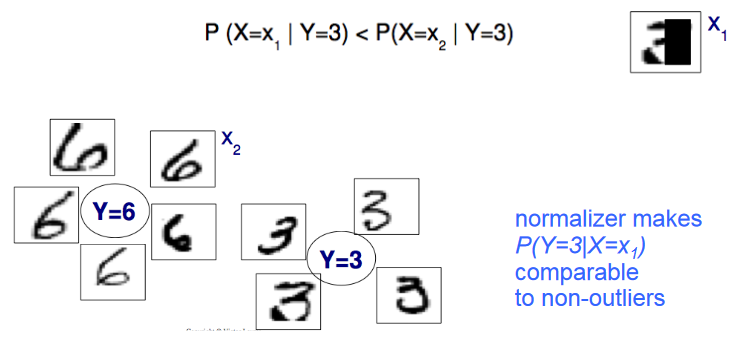
\includegraphics[width=0.6\linewidth,keepaspectratio]{nb2}
%\end{center}
%
%\begin{itemize}
%\item Its a digit recognition program. 
%\item Output class y is ether 3 or 6.
%\item Features are x1 and x2, say, x1 represent amount of ink.
%\end{itemize}
%
%\end{frame}
%
%
%%%%%%%%%%%%%%%%%%%%%%%%%%%%%%%%%%%%%%%%%%%%%%%%%%%%%%%%%%%
%\begin{frame}[fragile]\frametitle{Normalization Example}
%
%\begin{center}
%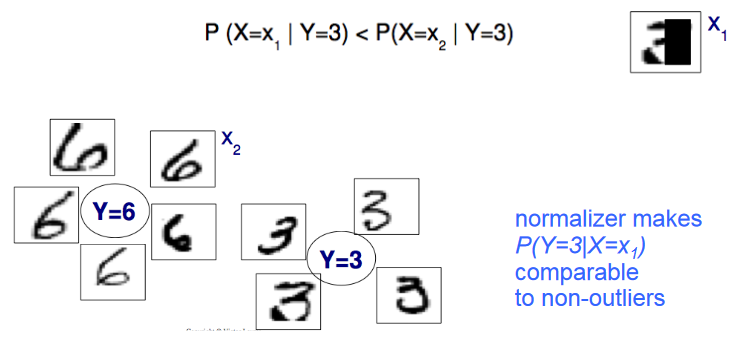
\includegraphics[width=0.6\linewidth,keepaspectratio]{nb2}
%\end{center}
%
%\begin{itemize}
%\item Look at outlier marked with x1.
%\item Its has so much ink (ie x1) so it does not know how to classify.
%\item So probability of this being classified as any class , 3 or 6, very very low.
%\item So x2 has more probability compare to x1, given that its a 3.
%
%\end{itemize}
%
%\end{frame}
%
%
%%%%%%%%%%%%%%%%%%%%%%%%%%%%%%%%%%%%%%%%%%%%%%%%%%%%%%%%%%%
%\begin{frame}[fragile]\frametitle{Normalization}
%\begin{itemize}
%\item What does Normalizer $P(x) = \sum P(x|y')P(y')$ do?
%\item It affects outlier. 
%\item Outlier has a low probability under every class.
%\item This being in denominator, boost the overall outcome of $P(Y=3|X=x_1)$ and sort of normalizes the outliers like any other
%\end{itemize}
%\begin{center}
%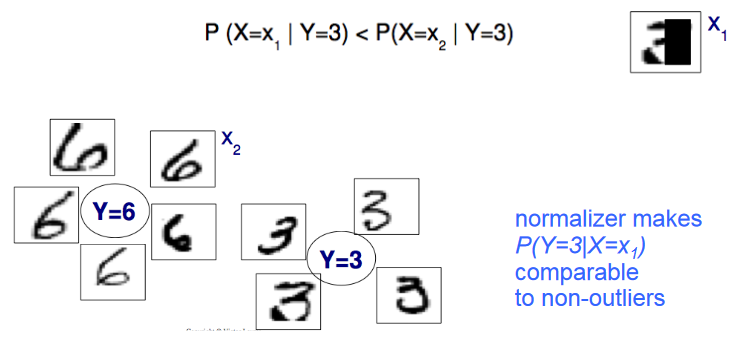
\includegraphics[width=0.6\linewidth,keepaspectratio]{nb2}
%\end{center}
%\end{frame}
%

% %%%%%%%%%%%%%%%%%%%%%%%%%%%%%%%%%%%%%%%%%%%%%%%%%%%%%%%%%%
% \begin{frame}[fragile]\frametitle{Independence assumption }
% \begin{itemize}
% \item When we need to compute $P(x|y)$, the x is actually many features.
% \item For Bitmaps 20x20, there are 400 x variables
% \item So there are $2^{400}$ patterns of x, 
% \item Probability of all these patterns is needed in deciding y=3 or y=6.
% \item That's too much!!
% \end{itemize}
% \end{frame}

%%%%%%%%%%%%%%%%%%%%%%%%%%%%%%%%%%%%%%%%%%%%%%%%%%%%%%%%%%
\begin{frame}[fragile]\frametitle{Independence assumption }
\begin{itemize}
\item Trick is to assume that all these x variables are independent, given y.
\item That makes combined probability as just multiplication of individual conditional probabilities.
\item So, it becomes sum of multiplications only
\begin{center}
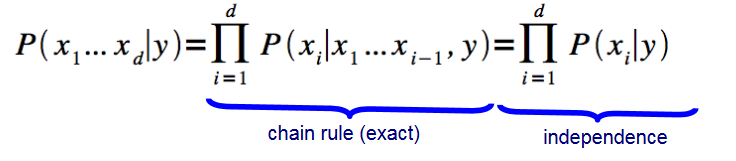
\includegraphics[width=\linewidth,keepaspectratio]{nb1}
\end{center}
\item Individual probabilities are: whats probability of a particular pixel being black given the digit is 3.
\item Multiply for all variables Xs.
\end{itemize}
\end{frame}

%%%%%%%%%%%%%%%%%%%%%%%%%%%%%%%%%%%%%%%%%%%%%%%%%%%%%%%%%%
\begin{frame}[fragile]\frametitle{Independence assumption }
\begin{itemize}
\item Joint probability of $Y$ and many features $X_1,X_2,X_3,\ldots,X_n$ can be expressed as the chain rule:

$P(Y,X_1,X_2,X_3,\ldots,X_n)$

$= P(X_1,X_2,X_3,\ldots,X_n|Y)P(Y)$

$= P(Y)P(X_1,Y)P(X_2|Y,X_1)P(X_3|Y,X_1,X_2)\ldots$

\item This is messy, but if we naively assume independence, then

$P(X_2|Y,X_1) = P(X_2|Y)$

$P(X_3|Y,X_1,X_2) = P(X_3|Y)$

$P(X_n|Y,X_1,X_2,\ldots) = P(X_n|Y)$

\end{itemize}
\end{frame}



%%%%%%%%%%%%%%%%%%%%%%%%%%%%%%%%%%%%%%%%%%%%%%%%%%%%%%%%%%%
%\begin{frame}[fragile]\frametitle{Independence assumption }
%\begin{itemize}
%\item Compute $P(x_1 \ldots x_n | y)$ for every observation $x_1 \ldots x_n$
%	\begin{itemize}
%	\item class-conditional ``counts'', based on training data
%	\item problem: may not have seen every $x_1 \ldots x_n$ for every $y$
%	\end{itemize}
%\item Probabilistic classification: most probable class given observation: $\hat{y} = arg~max_y P(y|x)$
%\item Idea: Assume $x_1 \ldots x_n$ conditionally independent given $y$
%\item So, it becomes sum of multiplications only
%\begin{center}
%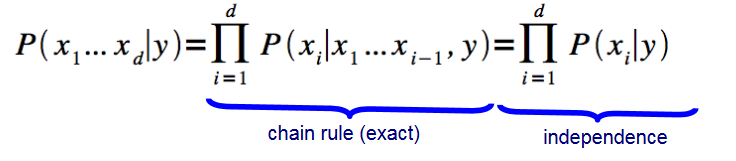
\includegraphics[width=\linewidth,keepaspectratio]{nb1}
%\end{center}
%\end{itemize}
%\end{frame}


%%%%%%%%%%%%%%%%%%%%%%%%%%%%%%%%%%%%%%%%%%%%%%%%%%%%%%%%%
\begin{frame}[fragile]\frametitle{Why is Bayes Classifier so popular?}
\begin{itemize}
\item Look at what it eventually comes down to. 
\item Just some counting and multiplication.
\item We can pre-compute all these terms, and so classifying becomes easy, quick and efficient. 
\end{itemize}
\end{frame}


%%%%%%%%%%%%%%%%%%%%%%%%%%%%%%%%%%%%%%%%%%%%%%%%%%%%%%%%%%%%%%%%%%%%%%%%%%%%%%%%%%
\begin{frame}[fragile]\frametitle{}
\begin{center}
{\Large Naive Bayes Example - Fruits Classification}
\end{center}
\end{frame}

%%%%%%%%%%%%%%%%%%%%%%%%%%%%%%%%%%%%%%%%%%%%%%%%%%%%%%%%%%
\begin{frame}[fragile]\frametitle{Example}
\begin{itemize}
\item So, let's say we have data on 1000 pieces of fruit. 
\item we know 3 features of each fruit, whether it's long or not, sweet or not and yellow or not
\item Outcome is the type: a Banana, Orange or some Other fruit.
\end{itemize}
\end{frame}


%%%%%%%%%%%%%%%%%%%%%%%%%%%%%%%%%%%%%%%%%%%%%%%%%%%%%%%%%%
\begin{frame}[fragile]\frametitle{Example}
\begin{center}
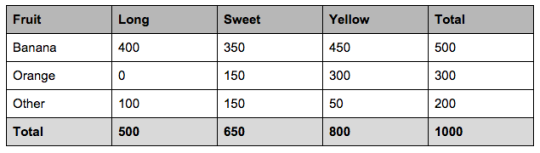
\includegraphics[width=0.6\linewidth,keepaspectratio]{nb8}
\end{center}
So from the table what do we already know?
\begin{itemize}
\item     50\% of the fruits are bananas
\item     30\% are oranges
\item     20\% are other fruits
\end{itemize}

\end{frame}

%%%%%%%%%%%%%%%%%%%%%%%%%%%%%%%%%%%%%%%%%%%%%%%%%%%%%%%%%%
\begin{frame}[fragile]\frametitle{Example}
More explicit table
\begin{center}
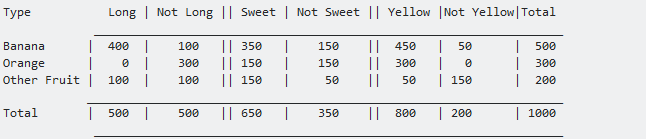
\includegraphics[width=\linewidth,keepaspectratio]{nb9}
\end{center}
This is our 'training set.' We will use this to predict the type of any new fruit we encounter.
\end{frame}

%%%%%%%%%%%%%%%%%%%%%%%%%%%%%%%%%%%%%%%%%%%%%%%%%%%%%%%%%%
\begin{frame}[fragile]\frametitle{Example}
We can pre-compute a lot of things about our fruit collection.
\begin{itemize}
\item     The so-called ``Prior'' probabilities. 
\item If we didn't know any of the fruit attributes, this would be our guess.
\item These are our base rates. P(Y).
\item P(Banana)      = 0.5 (500/1000)
\item  P(Orange)      = 0.3
\item  P(Other Fruit) = 0.2
\end{itemize}
\end{frame}

%%%%%%%%%%%%%%%%%%%%%%%%%%%%%%%%%%%%%%%%%%%%%%%%%%%%%%%%%%
\begin{frame}[fragile]\frametitle{Example}
Probability of ``Evidence''. P(X)
\begin{itemize}
\item P(Long)   = 0.5
\item P(Sweet)  = 0.65
\item P(Yellow) = 0.8
\end{itemize}
\end{frame}


%%%%%%%%%%%%%%%%%%%%%%%%%%%%%%%%%%%%%%%%%%%%%%%%%%%%%%%%%%
\begin{frame}[fragile]\frametitle{Example}
Based on our training set we can also say the following:
\begin{itemize}
\item From 500 bananas 400 (0.8) are Long, So $P(Long|Banana) = 0.8$
\item 350 (0.7) are Sweet. So, $P(Sweet|Banana) = 0.7$
\item 450 (0.9) are Yellow, So, $P(Yellow|Banana) = 0.9$
\end{itemize}
\end{frame}

%%%%%%%%%%%%%%%%%%%%%%%%%%%%%%%%%%%%%%%%%%%%%%%%%%%%%%%%%%
\begin{frame}[fragile]\frametitle{Example}
\begin{itemize}
\item Out of 300 oranges 0 are Long. So, $P(Long|Orange) = 0$. [Oranges are never long in all the fruit we have seen.]
\item 150 (0.5) are Sweet . So, $P(Sweet|Orange) = 0.5$
\item 300 (1) are Yellow.  So, $P(Yellow|Orange) = 1$
\end{itemize}
\end{frame}


%%%%%%%%%%%%%%%%%%%%%%%%%%%%%%%%%%%%%%%%%%%%%%%%%%%%%%%%%%
\begin{frame}[fragile]\frametitle{Example}
\begin{itemize}
\item From the remaining 200 fruits, 100 (0.5) are Long,  So $P(Long|Other) = 0.5$
\item 150 (0.75) are Sweet.  So $P(Sweet|Other) = 0.75$
\item 50 (0.25) are Yellow.  So $P(Yellow|Other) = 0.25$
\item Similarly, $P(Not Yellow|Other) = 0.75$ and so on
\end{itemize}
\end{frame}




%%%%%%%%%%%%%%%%%%%%%%%%%%%%%%%%%%%%%%%%%%%%%%%%%%%%%%%%%%
\begin{frame}[fragile]\frametitle{Example}
Testing
\begin{itemize}
\item Given the features of a piece of fruit and we need to predict the class
\item Test fruit is Long, Sweet and Yellow
\item The one (fruit) with the highest probability (score) being the winner.
\end{itemize}

\end{frame}

%%%%%%%%%%%%%%%%%%%%%%%%%%%%%%%%%%%%%%%%%%%%%%%%%%%%%%%%%%
\begin{frame}[fragile]\frametitle{Example}
\begin{center}
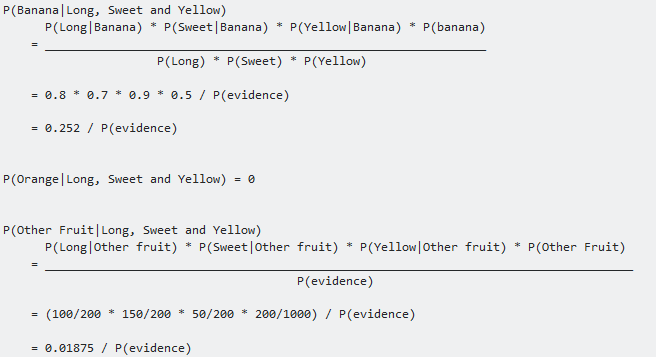
\includegraphics[width=\linewidth,keepaspectratio]{nb10}
\end{center}
By an overwhelming margin $(0.252 >> 0.01875)$, we classify this Sweet/Long/Yellow fruit as likely to be a Banana.
 \end{frame}


%%%%%%%%%%%%%%%%%%%%%%%%%%%%%%%%%%%%%%%%%%%%%%%%%%%%%%%%%%
%\begin{frame}[fragile]\frametitle{Predicted Probability Example}
%Scenario:
%
%\begin{itemize}
%\item A doctor knows that meningitis causes a stiff neck 50\% of the time
%\item Prior probability of any patient having meningitis is 1/50,000
%\item Prior probability of any patient having a stiff neck is 1/20
%\item If a patient has a stiff neck, what's the probability that they have meningitis?
%\item Apply Bayes' Rule:
%\begin{center}
%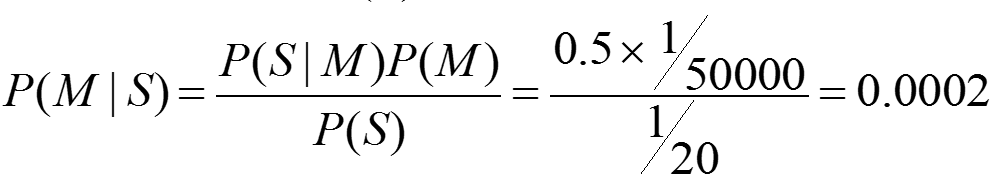
\includegraphics[width=0.5\linewidth,keepaspectratio]{nbneck}
%\end{center}
%\end{itemize}
%Very low probability
%
%\end{frame}

%%%%%%%%%%%%%%%%%%%%%%%%%%%%%%%%%%%%%%%%%%%%%%%%%%%%%%%%%%%%%%%%%%%%%%%%%%%%%%%%%%
\begin{frame}[fragile]\frametitle{}
\begin{center}
{\Large Naive Bayes Example - Loan Default}
\end{center}
\end{frame}

%%%%%%%%%%%%%%%%%%%%%%%%%%%%%%%%%%%%%%%%%%%%%%%%%%%%%%%%%%
\begin{frame}[fragile]\frametitle{Example}
\adjustbox{valign=t}{
\begin{minipage}{0.45\linewidth}

\begin{center}
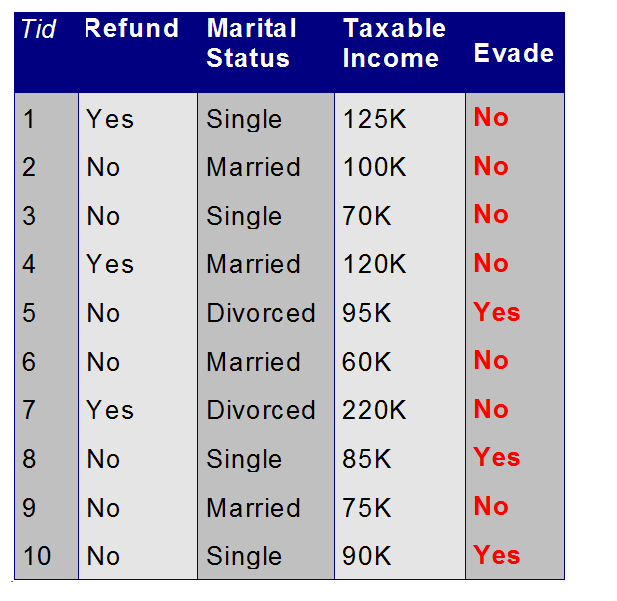
\includegraphics[width=\linewidth,keepaspectratio]{nbnecktble}
\end{center}

\end{minipage}
}
\hfill
\adjustbox{valign=t}{
\begin{minipage}{0.45\linewidth}

\begin{itemize}
\item Target class: Evade
\item Predictor variables: Refund, Status, Income
\item What is probability of Evade given the values of Refund, Status, Income?
\item $P(E|R,S,I)$
%\item Above .5? Predict YES, else predict NO.
\end{itemize}

\end{minipage}
}
\end{frame}


%%%%%%%%%%%%%%%%%%%%%%%%%%%%%%%%%%%%%%%%%%%%%%%%%%%%%%%%%%
\begin{frame}[fragile]\frametitle{Example}
\adjustbox{valign=t}{
\begin{minipage}{0.45\linewidth}

\begin{center}
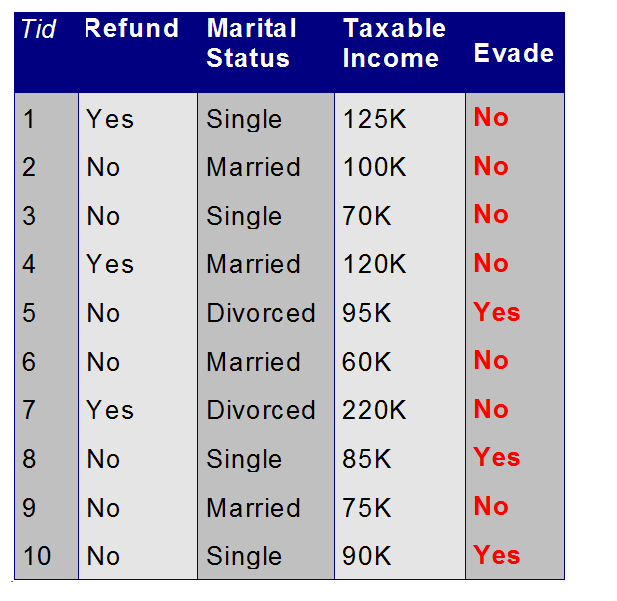
\includegraphics[width=\linewidth,keepaspectratio]{nbnecktble}
\end{center}

\end{minipage}
}
\hfill
\adjustbox{valign=t}{
\begin{minipage}{0.45\linewidth}

\begin{itemize}
\item Test instance is:
\begin{itemize}
\item Refund=Yes
\item Status=Married
\item Income=60K
\end{itemize}
\item Issue: we don't have any training example that these same three attributes values.
\item How to compute? $P(E|R,S,I)$
%\item What are values of R, S, I?

\end{itemize}

\end{minipage}
}
%Will need Multi feature Naive Bayes.
\end{frame}

%%%%%%%%%%%%%%%%%%%%%%%%%%%%%%%%%%%%%%%%%%%%%%%%%%%%%%%%%%%
%\begin{frame}[fragile]\frametitle{Naive Bayes Classifier}
%\begin{itemize}
%\item Why called naive?  Big assumption!
%\item Assumes that attributes (predictor variables) are conditionally independent. 
%\item No correlation: What is conditionally independent?
%\item Variable X is conditionally independent of Y if the following holds:
%\item $P(X|Y,Z) = P(X|Z)$
%\end{itemize}
%``given Z, what is the joint probability of X and Y?''
%\begin{center}
%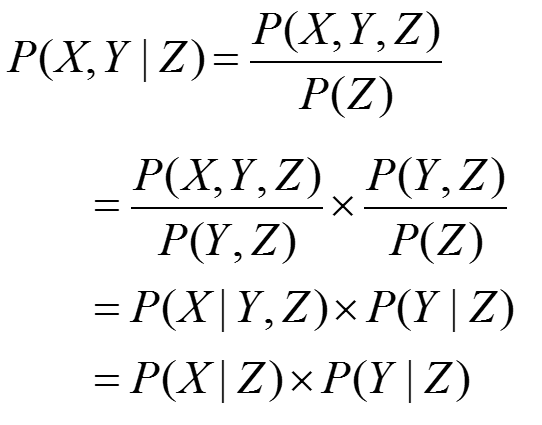
\includegraphics[width=0.3\linewidth,keepaspectratio]{condind}
%\end{center}
%\end{frame}
%
%%%%%%%%%%%%%%%%%%%%%%%%%%%%%%%%%%%%%%%%%%%%%%%%%%%%%%%%%%%
%\begin{frame}[fragile]\frametitle{Multi Feature Naive Bayes}
%\begin{center}
%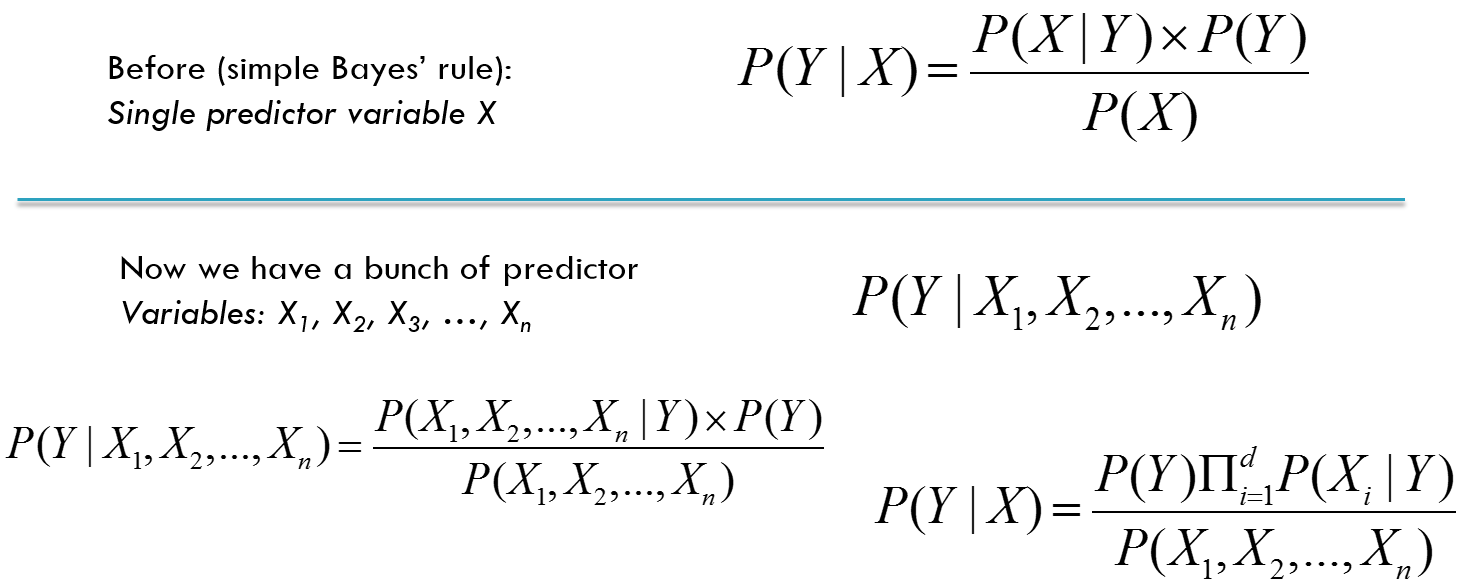
\includegraphics[width=\linewidth,keepaspectratio]{multinb}
%\end{center}
%
%\end{frame}
%
%%%%%%%%%%%%%%%%%%%%%%%%%%%%%%%%%%%%%%%%%%%%%%%%%%%%%%%%%%%
%\begin{frame}[fragile]\frametitle{Multi Feature Naive Bayes}
%\begin{center}
%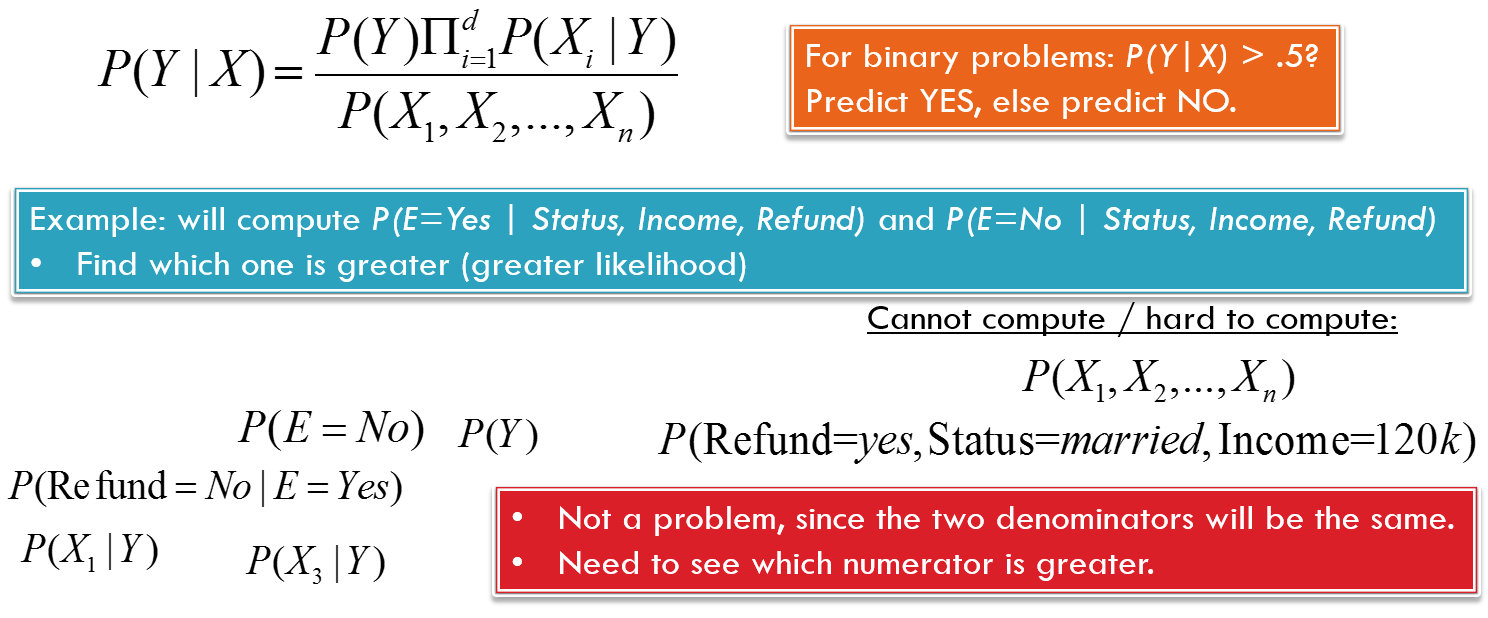
\includegraphics[width=\linewidth,keepaspectratio]{multinaiveb}
%\end{center}
%
%\end{frame}

%%%%%%%%%%%%%%%%%%%%%%%%%%%%%%%%%%%%%%%%%%%%%%%%%%%%%%%%%%
\begin{frame}[fragile]\frametitle{Estimating Prior Probabilities }
Class target $P(Y)$ (Count these from the table below)
\begin{center}
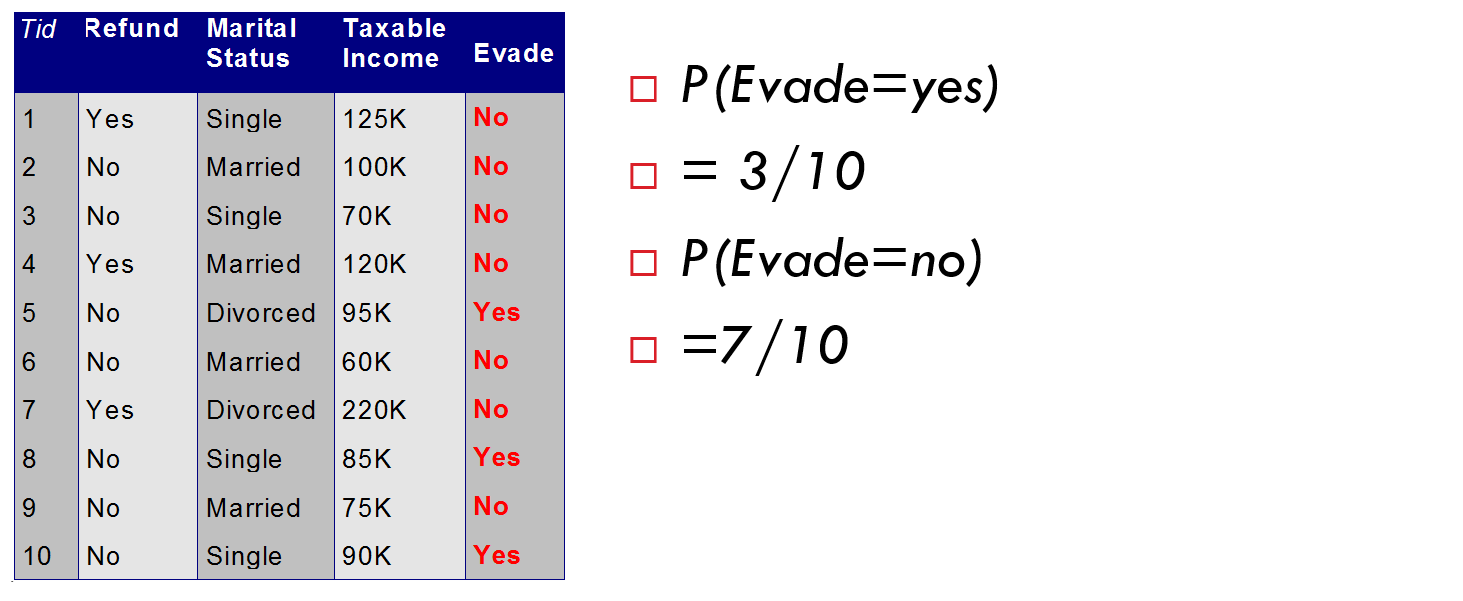
\includegraphics[width=\linewidth,keepaspectratio]{estnb1}
\end{center}
\end{frame}

%%%%%%%%%%%%%%%%%%%%%%%%%%%%%%%%%%%%%%%%%%%%%%%%%%%%%%%%%%
\begin{frame}[fragile]\frametitle{Estimating Prior Probabilities }
Categorical Attributes $P(X_1|Y)$ (Count these from the table below)
\begin{center}
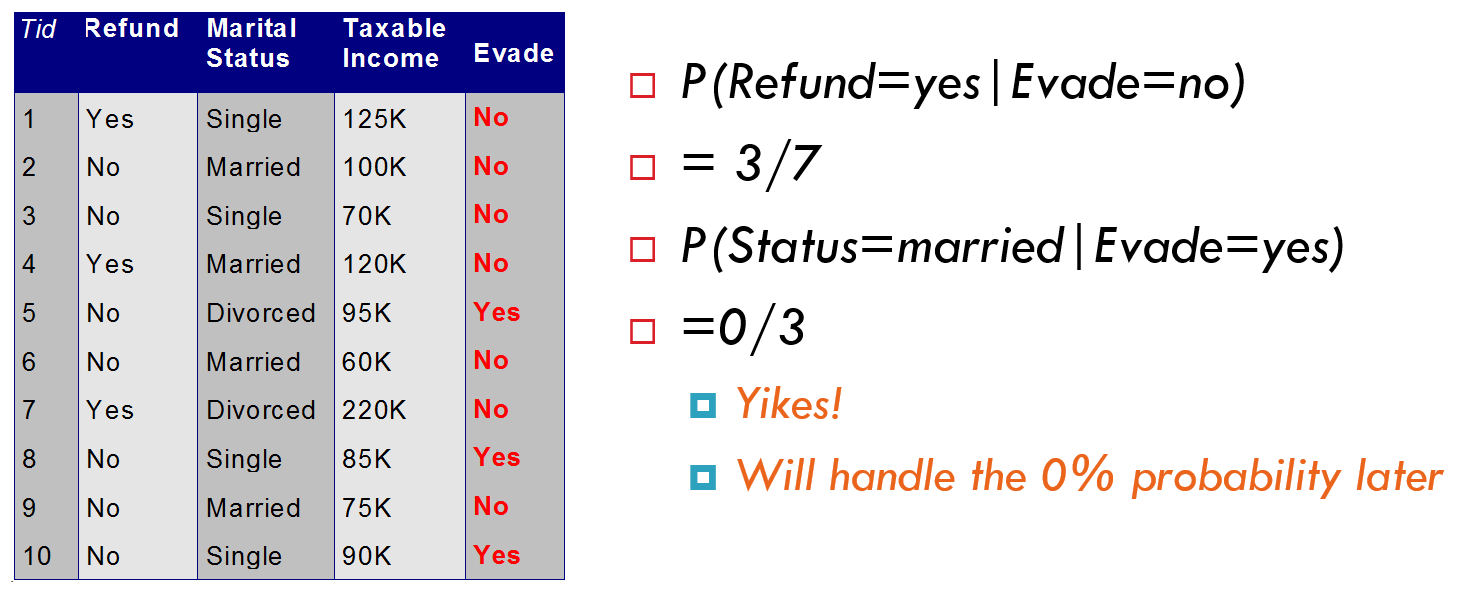
\includegraphics[width=\linewidth,keepaspectratio]{estnb2}
\end{center}
\end{frame}


%%%%%%%%%%%%%%%%%%%%%%%%%%%%%%%%%%%%%%%%%%%%%%%%%%%%%%%%%%
\begin{frame}[fragile]\frametitle{Estimating Prior Probabilities }
Continuous Attributes $P(X_1|Y)$ (Count these from the table below)
\begin{center}
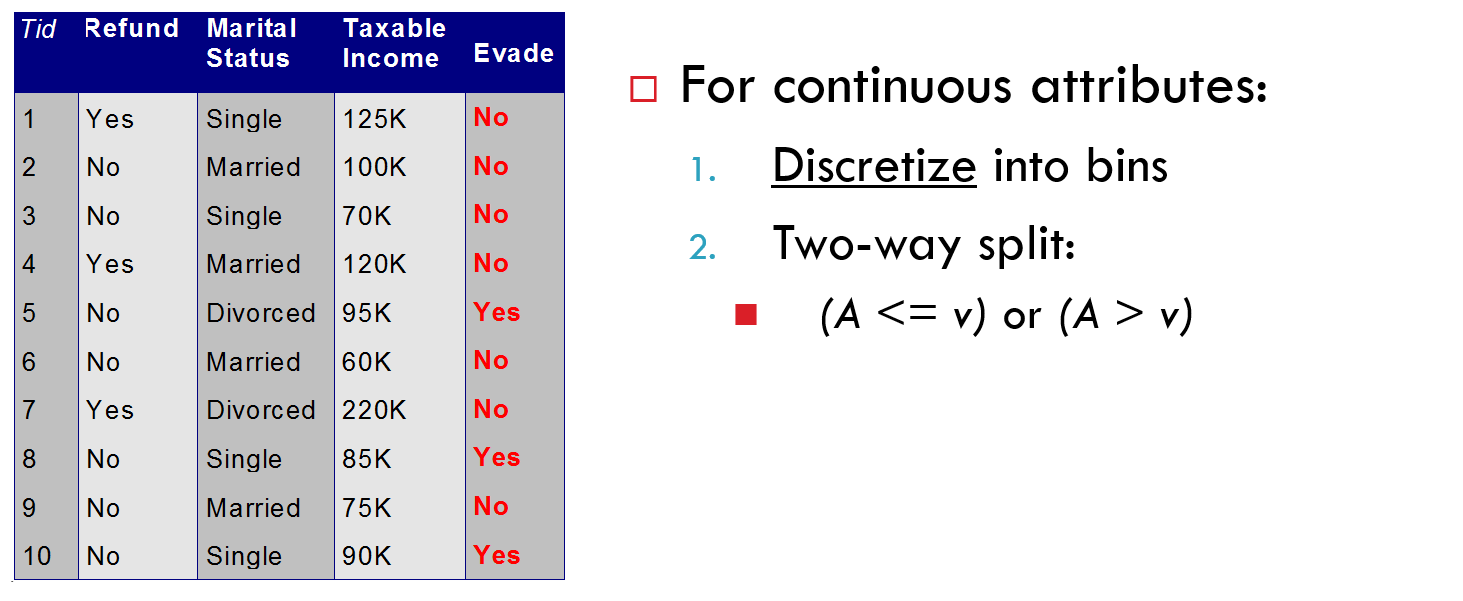
\includegraphics[width=\linewidth,keepaspectratio]{estnb3}
\end{center}
\end{frame}

%%%%%%%%%%%%%%%%%%%%%%%%%%%%%%%%%%%%%%%%%%%%%%%%%%%%%%%%%%
\begin{frame}[fragile]\frametitle{Estimating Prior Probabilities }
\begin{center}
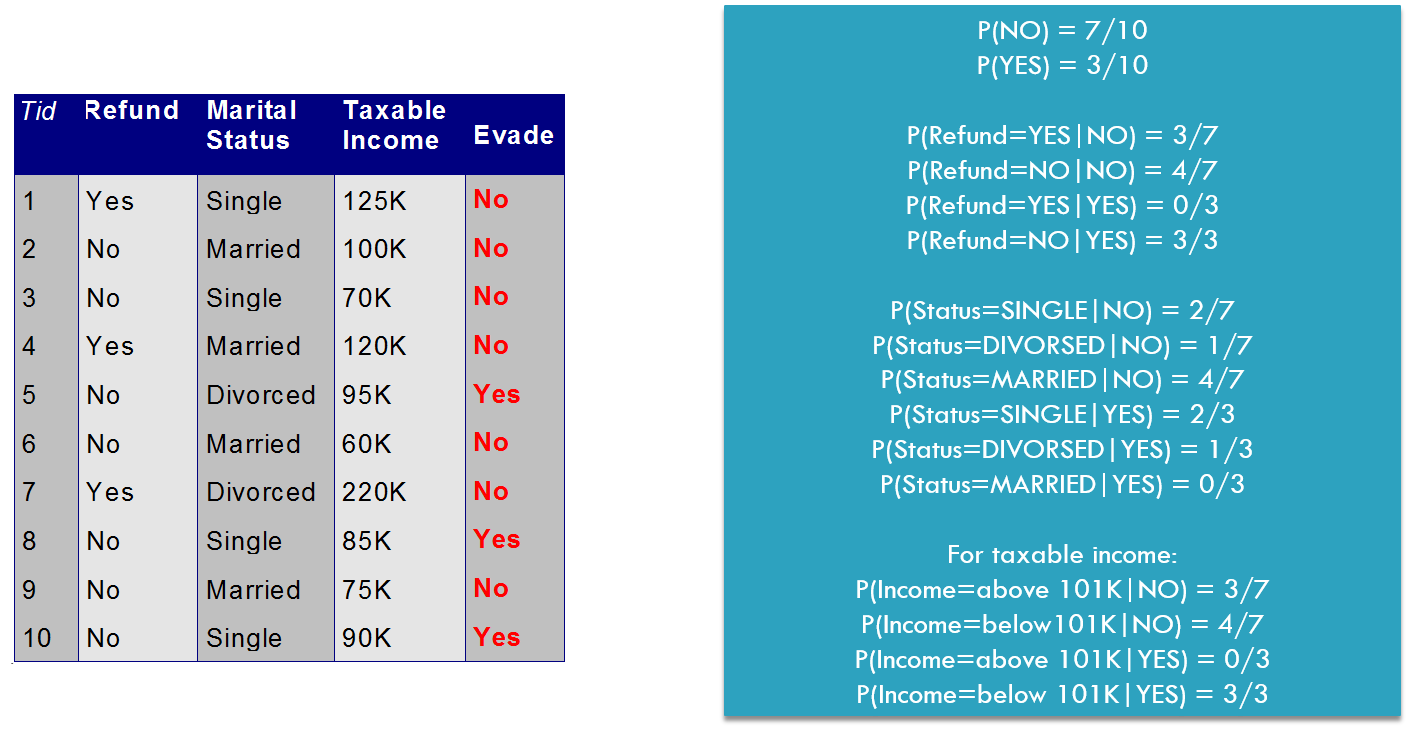
\includegraphics[width=\linewidth,keepaspectratio]{estnb4}
\end{center}
\end{frame}


%%%%%%%%%%%%%%%%%%%%%%%%%%%%%%%%%%%%%%%%%%%%%%%%%%%%%%%%%%
\begin{frame}[fragile]\frametitle{Estimating Prior Probabilities }
Test instance $X = (Refund = No, Married, Income = 75k)$
\begin{center}
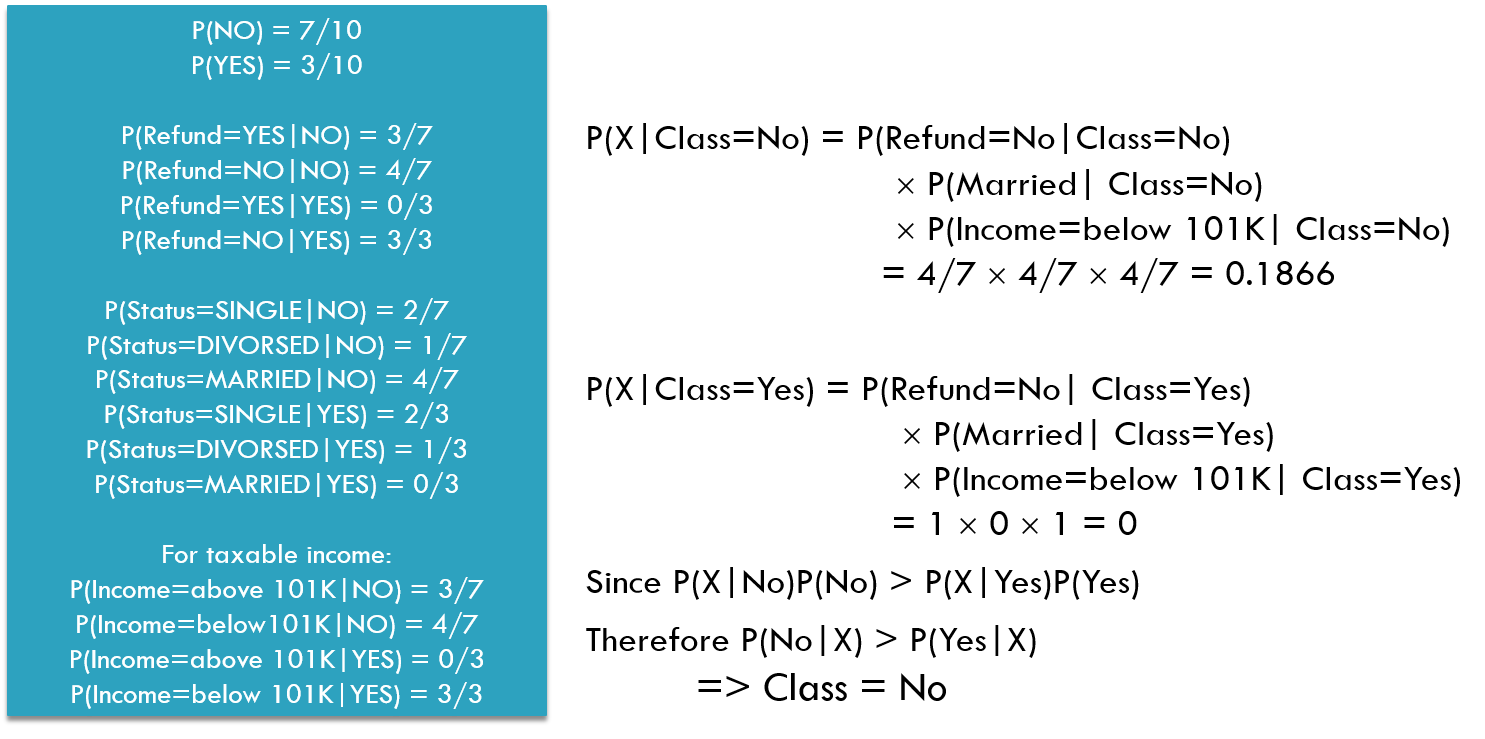
\includegraphics[width=\linewidth,keepaspectratio]{estnb5}
\end{center}
\end{frame}



%%%%%%%%%%%%%%%%%%%%%%%%%%%%%%%%%%%%%%%%%%%%%%%%%%%%%%%%%%%%
%\begin{frame}[fragile]\frametitle{Example}
%\begin{itemize}
%\item A training data set of weather and corresponding  target  variable  'Play'. 
%\item Now,  we  need  to  classify  whether  players  will  play  or  not based on weather condition.
%\item Step 1: Convert the data set to frequency table
%\item Step 2: Create Likelihood table by finding the probabilities like Overcast probability = 0.29 and probability of playing is 0.64.
%\item Step 3: Now, use Naive Bayesian equation to calculate the posterior probability for each class. The class with the highest posterior probability is the outcome of prediction.
%\end{itemize}
%\end{frame}
%
%%%%%%%%%%%%%%%%%%%%%%%%%%%%%%%%%%%%%%%%%%%%%%%%%%%%%%%%%%%%
%\begin{frame}[fragile]\frametitle{Example}
%\begin{center}
%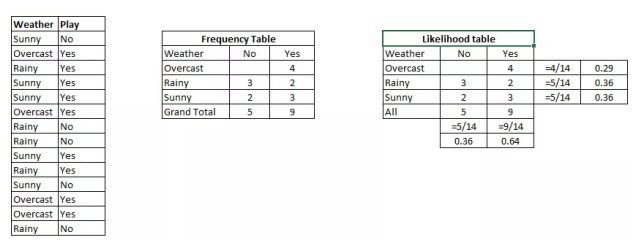
\includegraphics[width=\linewidth,keepaspectratio]{nb}
%\end{center}
%\end{frame}
%
%%%%%%%%%%%%%%%%%%%%%%%%%%%%%%%%%%%%%%%%%%%%%%%%%%%%%%%%%%%%
%\begin{frame}[fragile]\frametitle{Example}
%\begin{itemize}
%\item Problem: Players will pay if weather is sunny, is this statement is correct?
%\item $ P(Yes | Sunny) = P( Sunny | Yes) \times P(Yes) / P(Sunny)$
%\item $ P(Sunny |Yes) = 3/9 = 0.33, P(Sunny) = 5/14 = 0.36, P( Yes)= 9/14 = 0.64$
%\item $P(Yes | Sunny) = 0.33 \times 0.64 / 0.36 = 0.60$, which has higher probability.
%\item Naive Bayes uses a similar method to predict the probability of different class based on various
%attributes. 
%\item This algorithm is mostly used in text classification and with problems having multiple
%classes.
%\end{itemize}
%\end{frame}

%
%%%%%%%%%%%%%%%%%%%%%%%%%%%%%%%%%%%%%%%%%%%%%%%%%%%%%%%%%%%
%\begin{frame}[fragile]\frametitle{Smoothing of Conditional Probabilities}
%\begin{itemize}
%\item If one of the conditional probabilities is 0, then the entire product will be 0
%\item Idea: Instead use very small non-zeros values, such as 0.00001
%\begin{center}
%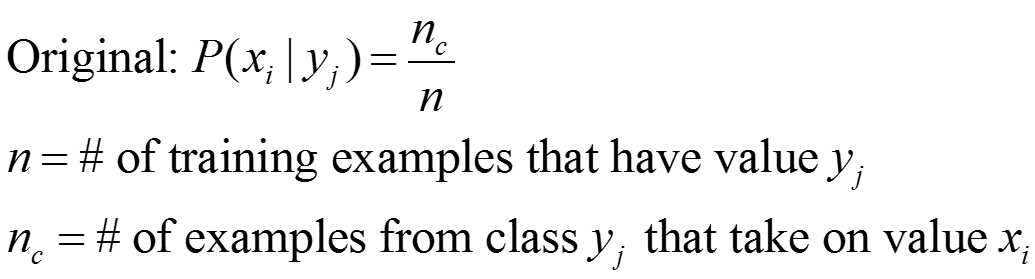
\includegraphics[width=\linewidth,keepaspectratio]{smooth}
%\end{center}
%\end{itemize}
%\end{frame}
%
%%%%%%%%%%%%%%%%%%%%%%%%%%%%%%%%%%%%%%%%%%%%%%%%%%%%%%%%%%%
%\begin{frame}[fragile]\frametitle{Smoothing of Conditional Probabilities}
%\begin{itemize}
%\item Idea: Instead use very small non-zeros values, such as 0.00001
%\begin{center}
%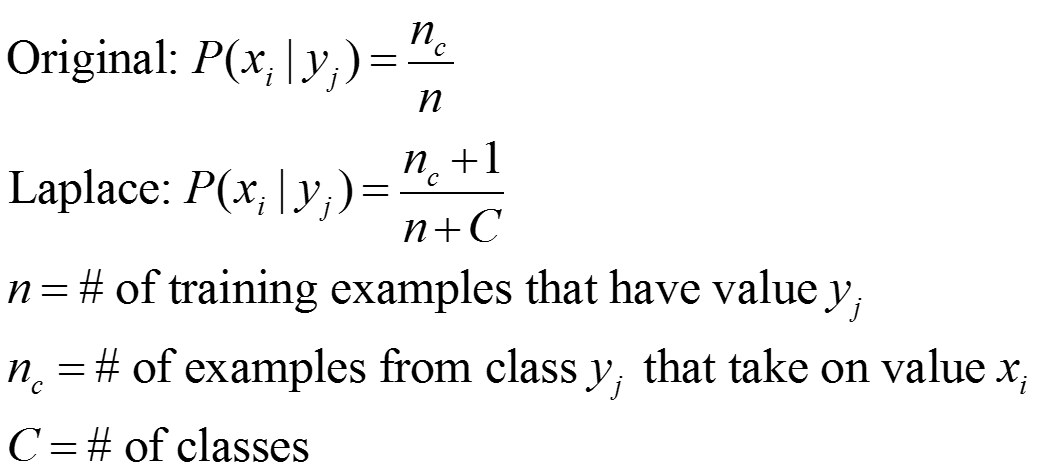
\includegraphics[width=\linewidth,keepaspectratio]{smooth1}
%\end{center}
%\end{itemize}
%\end{frame}
%
%%%%%%%%%%%%%%%%%%%%%%%%%%%%%%%%%%%%%%%%%%%%%%%%%%%%%%%%%%%
%\begin{frame}[fragile]\frametitle{Laplace Smoothing }
%Test instance $X = (Refund = No, Married, Income = 75k)$
%\begin{center}
%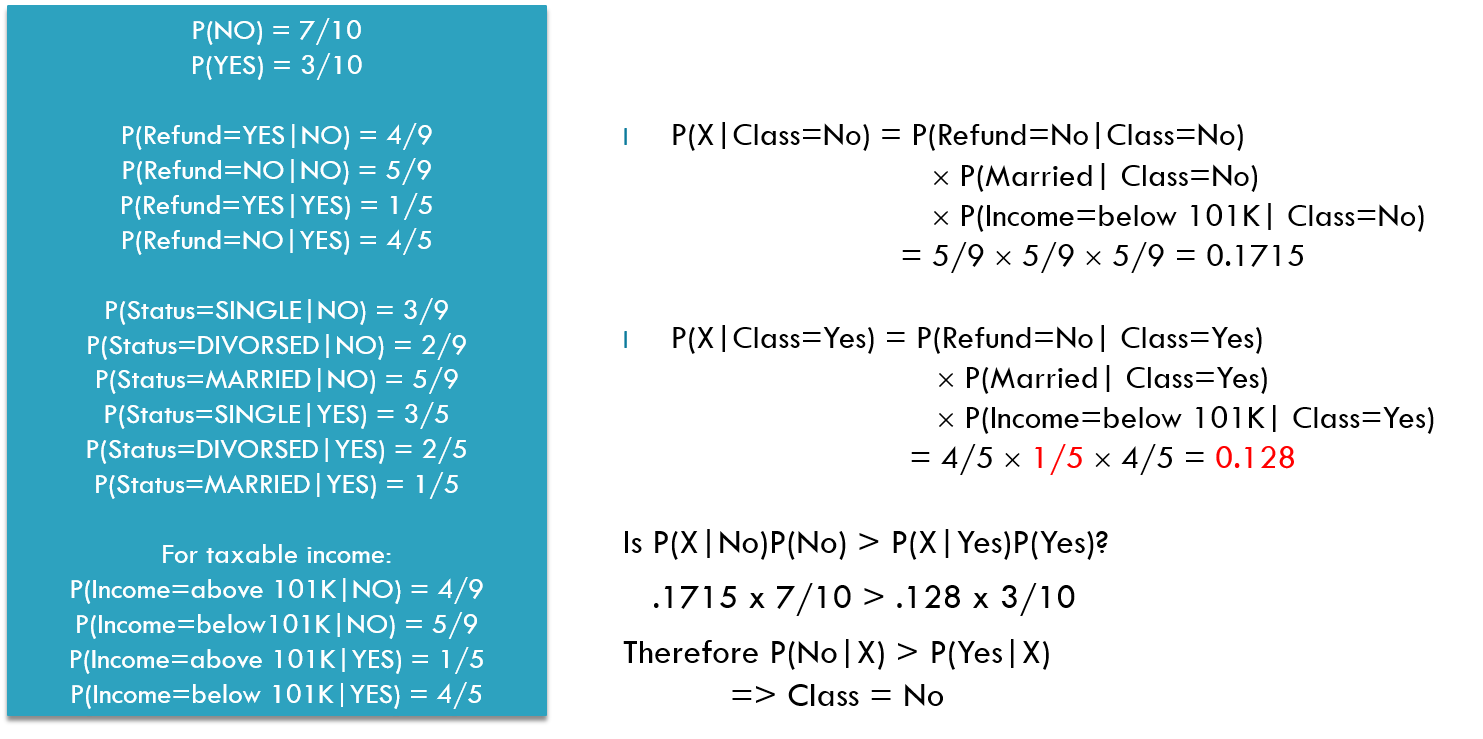
\includegraphics[width=\linewidth,keepaspectratio]{smooth2}
%\end{center}
%\end{frame}
%
%%%%%%%%%%%%%%%%%%%%%%%%%%%%%%%%%%%%%%%%%%%%%%%%%%%%%%%%%%%
%\begin{frame}[fragile]\frametitle{Characteristics of Naive Bayes Classifier}
%\begin{itemize}
%\item Robust to isolated noise: Noise is averaged out by estimating the conditional probabilities from data
%\item Handling missing values: Simply ignore them when estimating the probabilities
%\item Robust to irrelevant attributes: If Xi is an irrelevant attribute, then P(Xi|Y) becomes almost uniformly distributed
%\begin{itemize}
%\item P(Refund=Yes|YES)=0.5
%\item P(Refund=Yes|NO)=0.5
%\end{itemize}
%\item Independence assumption may not hold for some attributes
%\item Correlated attributes can degrade performance of naïve Bayes
%\item But, naive Bayes (for such a simple model), still works surprisingly well even when there is some correlation between attributes
%
%\end{itemize}
%\end{frame}
%
%%%%%%%%%%%%%%%%%%%%%%%%%%%%%%%%%%%%%%%%%%%%%%%%%%%%%%%%%%%%
%\begin{frame}[fragile]\frametitle{Example}
%\begin{center}
%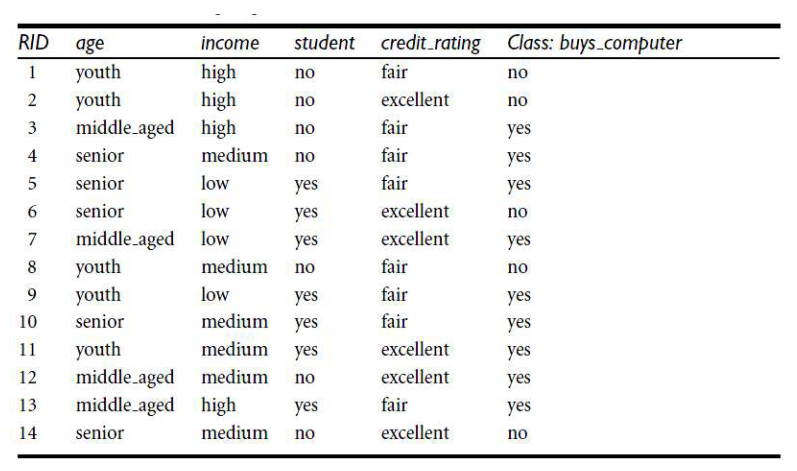
\includegraphics[width=\linewidth,keepaspectratio]{buycomp1}
%\end{center}
%\end{frame}
%
%%%%%%%%%%%%%%%%%%%%%%%%%%%%%%%%%%%%%%%%%%%%%%%%%%%%%%%%%%%%
%\begin{frame}[fragile]\frametitle{Example}
%\begin{center}
%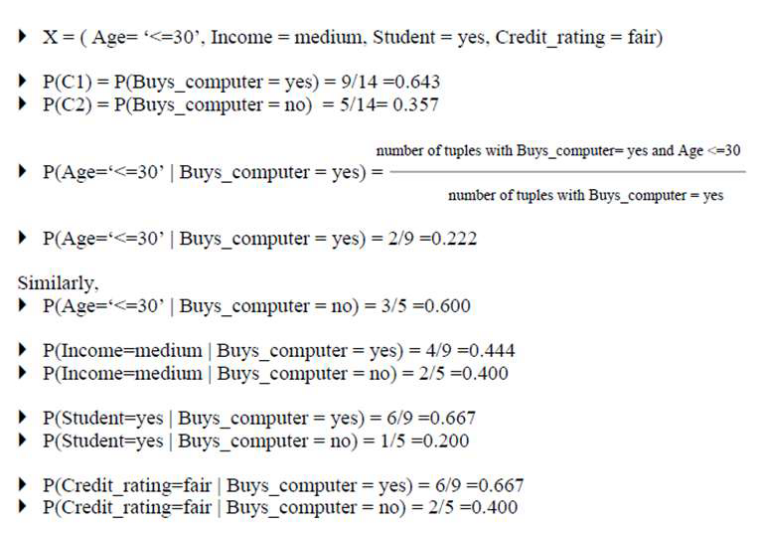
\includegraphics[width=\linewidth,keepaspectratio]{buycomp2}
%\end{center}
%\end{frame}

%%%%%%%%%%%%%%%%%%%%%%%%%%%%%%%%%%%%%%%%%%%%%%%%%%%%%%%%%%%%%%%%%%%%%%%%%%%%%%%%%%
\begin{frame}[fragile]\frametitle{}
\begin{center}
{\Large Naive Bayes Classification with Continuous Input Variables}
\end{center}
\end{frame}


%%%%%%%%%%%%%%%%%%%%%%%%%%%%%%%%%%%%%%%%%%%%%%%%%%%%%%%%%%
\begin{frame}[fragile]\frametitle{Continuous Variable Example}
\begin{itemize}
\item    Features: Height and Weight
\item Outcome: class children, adults
\end{itemize}
\begin{center}
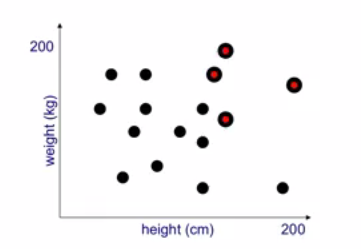
\includegraphics[width=0.5\linewidth,keepaspectratio]{nb11}
\end{center}
\end{frame}

%%%%%%%%%%%%%%%%%%%%%%%%%%%%%%%%%%%%%%%%%%%%%%%%%%%%%%%%%%
\begin{frame}[fragile]\frametitle{Continuous Variable Example}
Compute priors, for children and Adults
\begin{center}
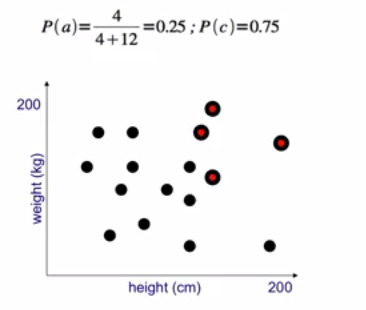
\includegraphics[width=0.5\linewidth,keepaspectratio]{nb12}
\end{center}
\end{frame}

%%%%%%%%%%%%%%%%%%%%%%%%%%%%%%%%%%%%%%%%%%%%%%%%%%%%%%%%%%
\begin{frame}[fragile]\frametitle{Continuous Variable Example}
\begin{itemize}
\item  Now, within children (black dots), look at only Height for now.
\item  That would be projection of black dots on X axis.
\end{itemize}
\begin{center}
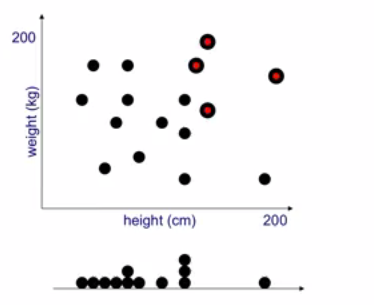
\includegraphics[width=0.5\linewidth,keepaspectratio]{nb13}
\end{center}
\begin{itemize}
\item  One child is really tall.
\item Rest are sort of together on smaller values.
\end{itemize}
\end{frame}

%%%%%%%%%%%%%%%%%%%%%%%%%%%%%%%%%%%%%%%%%%%%%%%%%%%%%%%%%%
\begin{frame}[fragile]\frametitle{Continuous Variable Example}
\begin{center}
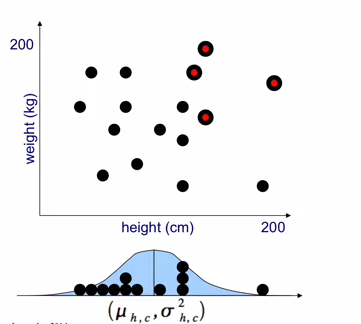
\includegraphics[width=0.5\linewidth,keepaspectratio]{nb14}
\end{center}
\begin{itemize}
\item  Modeling the Histogram with Gaussian (as this is continuous data!!)
\item Its not a good fit, but Gaussian is easy to handle.
\end{itemize}
\end{frame}

%%%%%%%%%%%%%%%%%%%%%%%%%%%%%%%%%%%%%%%%%%%%%%%%%%%%%%%%%%
\begin{frame}[fragile]\frametitle{Continuous Variable Example}
\begin{itemize}
\item  Same thing for Weights.
\item These, both, Gaussians are independent.
\item Their respective values can be multiplied
\end{itemize}
\begin{center}
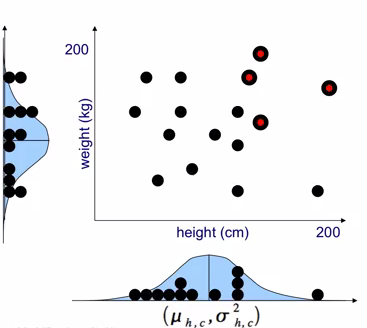
\includegraphics[width=0.5\linewidth,keepaspectratio]{nb15}
\end{center}
\end{frame}

%%%%%%%%%%%%%%%%%%%%%%%%%%%%%%%%%%%%%%%%%%%%%%%%%%%%%%%%%%
\begin{frame}[fragile]\frametitle{Continuous Variable Example}
\begin{itemize}
\item Cross plot with contours (iso values)
\item Peak in the middle,where Height and Weights are max.
\item This is for Children
\end{itemize}
\begin{center}
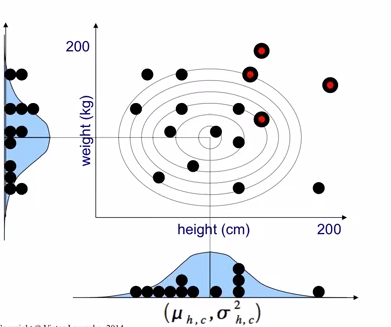
\includegraphics[width=0.5\linewidth,keepaspectratio]{nb17}
\end{center}
\end{frame}

%%%%%%%%%%%%%%%%%%%%%%%%%%%%%%%%%%%%%%%%%%%%%%%%%%%%%%%%%%
\begin{frame}[fragile]\frametitle{Continuous Variable Example}
\begin{itemize}
\item Adding Gaussian plot for Adults as well
\item You can start seeing separate regions, ie classification.
\item Thats the Gaussian Naive Bayes model
\end{itemize}
\begin{center}
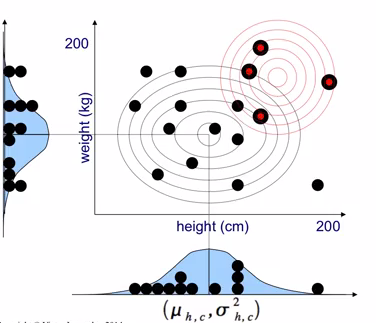
\includegraphics[width=0.5\linewidth,keepaspectratio]{nb18}
\end{center}
\end{frame}


%%%%%%%%%%%%%%%%%%%%%%%%%%%%%%%%%%%%%%%%%%%%%%%%%%%%%%%%%%
\begin{frame}[fragile]\frametitle{Continuous Variable Example}
\begin{itemize}
\item A test point needs to see if its a child or an adult
\item He has height as well as weight
\item Plug those in for Gaussian of Height and Weight and for both Adults and Children
\item Combine them using Bayes rule
\end{itemize}
\end{frame}

%%%%%%%%%%%%%%%%%%%%%%%%%%%%%%%%%%%%%%%%%%%%%%%%%%%%%%%%%%
\begin{frame}[fragile]\frametitle{Continuous Variable Example}
\begin{center}
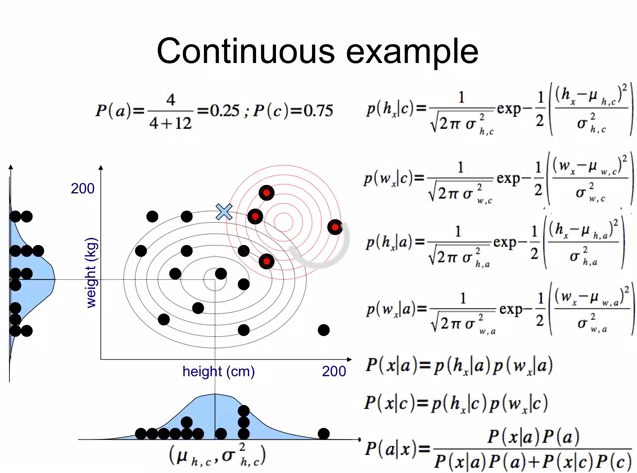
\includegraphics[width=0.8\linewidth,keepaspectratio]{nb19}
\end{center}
\end{frame}






%%%%%%%%%%%%%%%%%%%%%%%%%%%%%%%%%%%%%%%%%%%%%%%%%%%%%%%%%
\begin{frame}[fragile]\frametitle{Pros and cons}
Advantages
\begin{itemize}
\item     It's relatively simple to understand and build
\item     It's easily trained, even with a small data-set
\item     It's fast!
\item     It's not sensitive to irrelevant features
\end{itemize}
Disadvantages
\begin{itemize}
\item     It assumes every feature is independent, which isn't always the case
\end{itemize}
\end{frame}




%%%%%%%%%%%%%%%%%%%%%%%%%%%%%%%%%%%%%%%%%%%%%%%%%%%%%%%%%%
\begin{frame}[fragile]\frametitle{Naive Bayes (Summary)}
\begin{itemize}
\item Classification based on Bayes theorem
\item Assumption of independence between predictors.
\item That is a too `naive' assumption to make.
\item Naive Bayesian model is easy to build and particularly useful for very large data sets. 
\item Along with simplicity, Naive Bayes is known to outperform even highly sophisticated classification methods.
\end{itemize}
\end{frame}


%%%%%%%%%%%%%%%%%%%%%%%%%%%%%%%%%%%%%%%%%%%%%%%%%%%%%%%%%%
\begin{frame}[fragile]\frametitle{Naive Bayes (Summary)}
\begin{itemize}
\item In many datasets, relationship between attributes and class variable is non-deterministic.
\item Why?
	\begin{itemize}
	\item Noisy data
	\item Confounding and interaction of factors
	\item Relevant variables not included in the data
	\end{itemize}

\item Scenario
	\begin{itemize}
	\item Risk of heart disease based on individual's diet and workout frequency
	\item Most people who ``work out'' and have a healthy diet don't get heart disease. Yet, some healthy individuals still do: Smoking, alcohol abuse
	\end{itemize}
\end{itemize}
\end{frame}